%% GENERATED by rbrl/gen_figs.py from results/T6_per_window.csv.
%% Do not edit by hand; regenerate.
\begin{figure}[t]
\centering
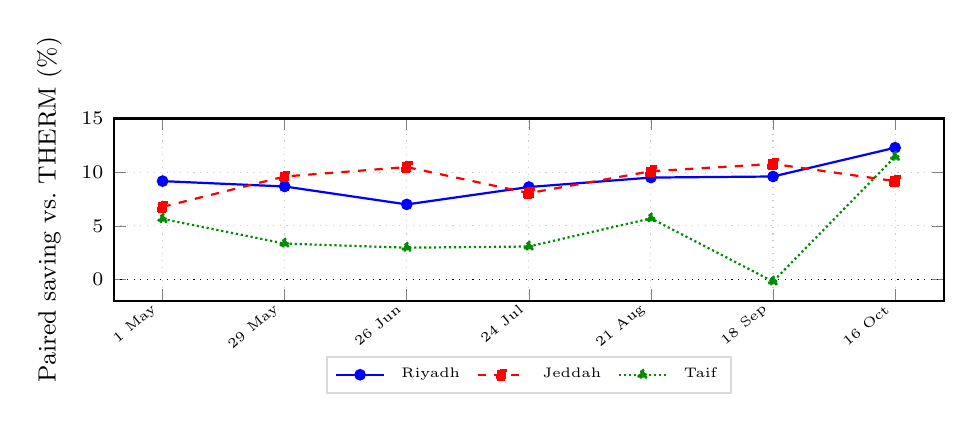
\begin{tikzpicture}
\begin{axis}[
  width=\linewidth, height=3.9cm,
  grid=major, grid style={dotted,gray!40},
  tick label style={font=\scriptsize},
  label style={font=\small},
  legend style={at={(0.5,-0.30)},anchor=north,legend columns=3,
                font=\tiny,draw=gray!30,column sep=4pt},
  thick,
  xmin=0.6, xmax=7.4, xtick={1,...,7},
  xticklabels={1 May,29 May,26 Jun,24 Jul,21 Aug,18 Sep,16 Oct},
  xticklabel style={font=\tiny,rotate=40,anchor=east},
  ylabel={Paired saving vs.\ THERM (\%)},
  ymin=-2, ymax=15,
]
\addplot[black,dotted,thin,forget plot] coordinates{(0.6,0)(7.4,0)};
\addplot[blue,thick,mark=*,mark size=1.7pt]
  coordinates{(1,9.16)(2,8.66)(3,6.99)(4,8.61)(5,9.49)(6,9.59)(7,12.27)};
\addlegendentry{Riyadh}
\addplot[red,thick,dashed,mark=square*,mark size=1.7pt]
  coordinates{(1,6.76)(2,9.59)(3,10.47)(4,8.04)(5,10.08)(6,10.76)(7,9.16)};
\addlegendentry{Jeddah}
\addplot[green!55!black,thick,densely dotted,mark=triangle*,mark size=2pt]
  coordinates{(1,5.64)(2,3.34)(3,2.96)(4,3.07)(5,5.69)(6,-0.19)(7,11.43)};
\addlegendentry{Taif}
\end{axis}
\end{tikzpicture}
\caption{Paired saving on each held-out window, tariff in force. Each window is
differenced against its \emph{own} baseline run, because the baseline's cost
varies by a factor of $1.9$ across the season; a saving quoted against the
seasonal mean would carry a spurious dispersion. Riyadh and Jeddah are stable
across the season ($\pm1.6$ and $\pm1.4$ points); Taif, the mild-climate site,
is not, and includes one window at $-0.2\%$ where the tuned rule is no better
than the baseline. Source: the project repository
(Section~\ref{sec:data}).}
\label{fig:season}
\end{figure}
